\documentclass[aspectratio=169]{beamer}

% ---------------------------------------------------------------------------
% Paquetes
% ---------------------------------------------------------------------------
\usepackage[utf8]{inputenc}
\usepackage[T1]{fontenc}
\usepackage[spanish,es-noquoting]{babel}
\usepackage{graphicx}
\usepackage{booktabs}
\usepackage{array}
\usepackage{colortbl}
\usepackage{xcolor}
\usepackage{amsmath}
\usepackage{multicol}

\graphicspath{{../informe_imagenes/}}

% ---------------------------------------------------------------------------
% Tema y colores
% ---------------------------------------------------------------------------
\usetheme{Madrid}
\usecolortheme{default}
\setbeamertemplate{headline}{}
\setbeamertemplate{navigation symbols}{}

\definecolor{ProjBlue}{RGB}{27,58,102}
\definecolor{ProjOrange}{RGB}{224,158,73}
\definecolor{ProjLight}{RGB}{233,238,246}

\setbeamercolor{structure}{fg=ProjBlue}
\setbeamercolor{title}{fg=white,bg=ProjBlue}
\setbeamercolor{frametitle}{fg=white,bg=ProjBlue}
\setbeamercolor{block title}{fg=white,bg=ProjBlue}
\setbeamercolor{block body}{fg=black,bg=ProjLight}
\setbeamercolor{alerted text}{fg=ProjOrange}
\setbeamercolor{footline}{fg=ProjBlue,bg=ProjLight}
\setbeamerfont{footline}{size=\tiny}
\setbeamertemplate{footline}{%
  \leavevmode
  \hbox{\begin{beamercolorbox}[wd=1\paperwidth,ht=2.4ex,dp=1.2ex,leftskip=1em,rightskip=1em]{footline}
    \usebeamerfont{footline}%
    Recuperaci\'on de im\'agenes de edificios \hfill SIFT / BoVW / VLAD / Re-ranking \hfill \insertframenumber{}/\inserttotalframenumber
  \end{beamercolorbox}}%
}

\newcommand{\ideaclave}[1]{%
  \vfill
  \begin{beamercolorbox}[wd=\textwidth,sep=0.35em]{block body}
    \small\textbf{Idea clave:} #1
  \end{beamercolorbox}
}

% ---------------------------------------------------------------------------
% Datos de portada
% ---------------------------------------------------------------------------
\title[Retrieval de edificios: SIFT/BoVW/VLAD]{Recuperaci\'on de im\'agenes de edificios con m\'etodos cl\'asicos}
\subtitle{SIFT, BoVW, VLAD y re-ranking sobre Oxford Buildings y Paris Buildings}
\author{Diego Quispe \and Brigitte Rojas \and Alvaro Garcia \and Sofia Salazar \and Marcelino Maita}
\institute{Visi\'on por Computador \\ Proyecto 1}
\date{\today}

\begin{document}

% ============================================================================
\begin{frame}[plain]
  \titlepage
\end{frame}

% ============================================================================
\begin{frame}{Idea central}
  \begin{center}
    \Large
    \alert{SIFT + BoVW} es un buen \emph{baseline}, pero pierde la distribuci\'on\\
    de los descriptores. \alert{VLAD} conserva esa informaci\'on y el\\
    \alert{re-ranking} mejora el orden final del ranking.
  \end{center}
  \vspace{1em}
  \begin{center}
    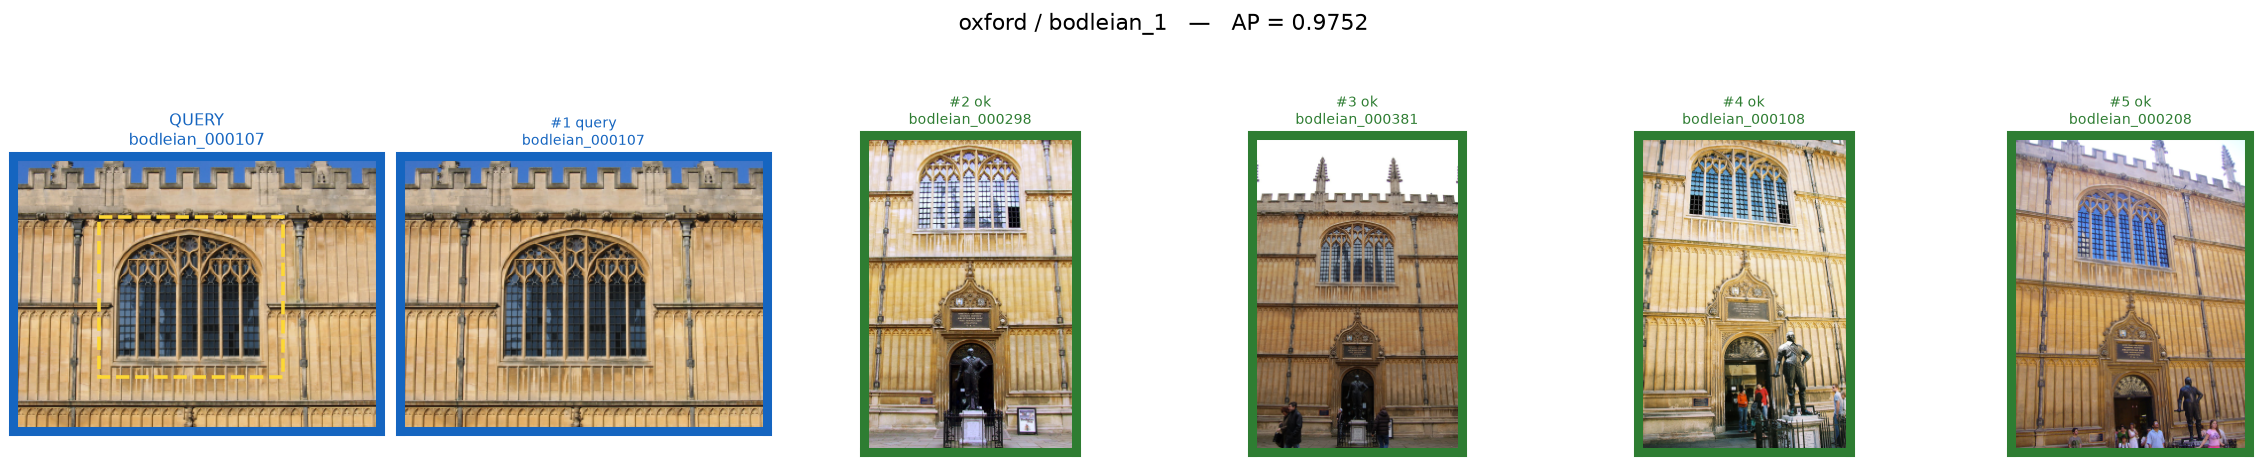
\includegraphics[width=0.95\textwidth]{11_qualitative/vlad_mejor_pipeline_dba_difusion/mejor_0.975_oxford_bodleian_1.png}
  \end{center}
  \begin{center}
    \footnotesize Consulta (izquierda, en azul) y resultados recuperados (verde = relevante) --- pipeline final, AP~=~0.975
  \end{center}
\end{frame}

% ============================================================================
\begin{frame}{Agenda}
  \begin{columns}[T]
    \begin{column}{0.5\textwidth}
      \begin{enumerate}
        \item Problema y dataset
        \item Pipeline general
        \item SIFT y RootSIFT
        \item BoVW y vocabulario visual
        \item Representaciones comparadas
        \item VLAD y PCA whitening
      \end{enumerate}
    \end{column}
    \begin{column}{0.5\textwidth}
      \begin{enumerate}
        \setcounter{enumi}{6}
        \item Similitud y re-ranking
        \item Evaluaci\'on
        \item Oxford vs.\ Paris
        \item Casos exitosos y fallos
        \item Conclusiones
      \end{enumerate}
    \end{column}
  \end{columns}
\end{frame}

% ============================================================================
\begin{frame}{Problema y dataset}
  \begin{columns}[T]
    \begin{column}{0.45\textwidth}
      \textbf{Oxford Buildings}
      \begin{itemize}
        \item 5{,}062 im\'agenes
        \item 11 landmarks, 55 queries
      \end{itemize}
      \vspace{0.5em}
      \textbf{Paris Buildings}
      \begin{itemize}
        \item 6{,}412 im\'agenes
        \item 11 landmarks, 55 queries
      \end{itemize}
      \vspace{0.5em}
      Cada query tiene imagen, \emph{bounding box} y listas \texttt{good}, \texttt{ok} y \texttt{junk}.
    \end{column}
    \begin{column}{0.55\textwidth}
      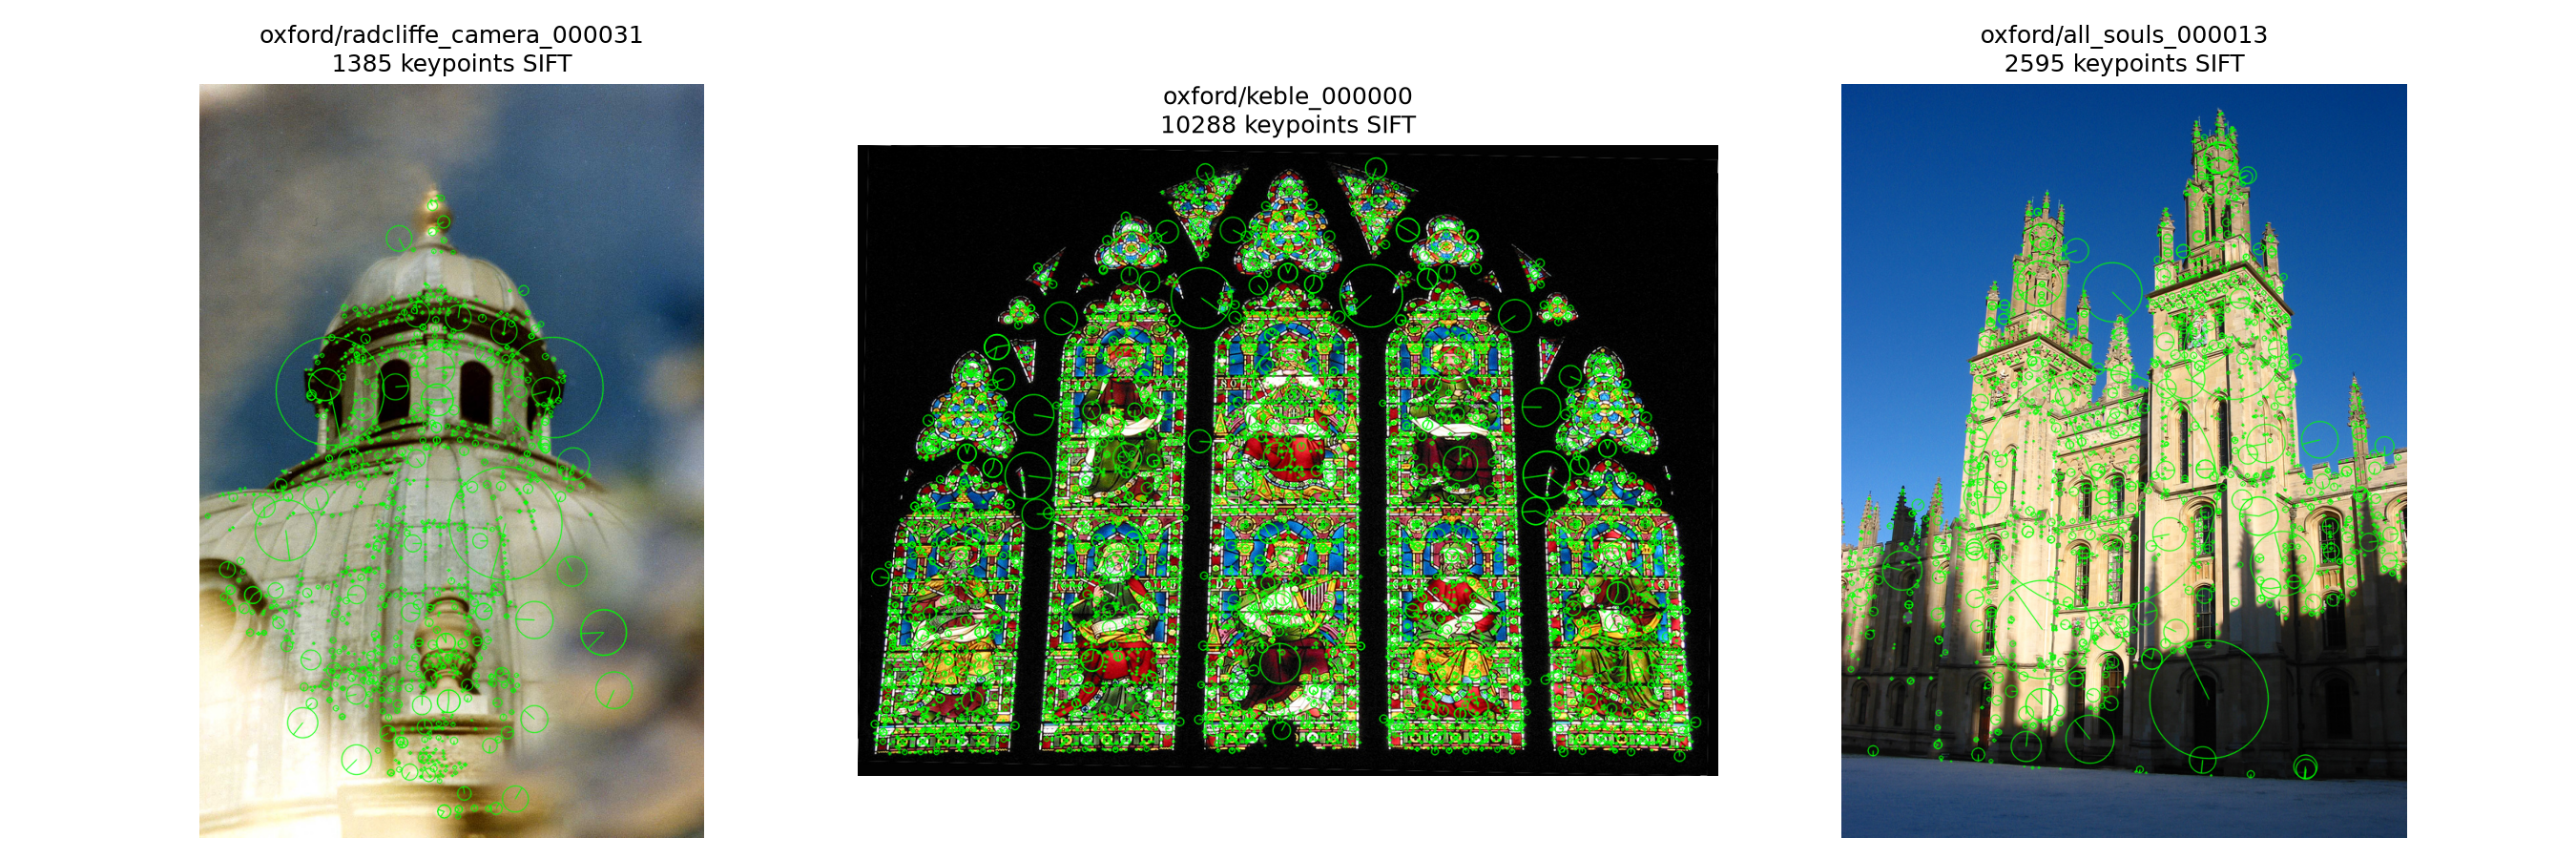
\includegraphics[width=\textwidth]{01_sift_keypoints/sift_keypoints_ejemplos.png}
    \end{column}
  \end{columns}
  \ideaclave{La dificultad no es solo encontrar la misma fachada: hay vegetaci\'on, cielo, otras fachadas y cambios fuertes de perspectiva.}
\end{frame}

% ============================================================================
\begin{frame}{Pipeline general (1/2): extracci\'on de descriptores}
  \centering
  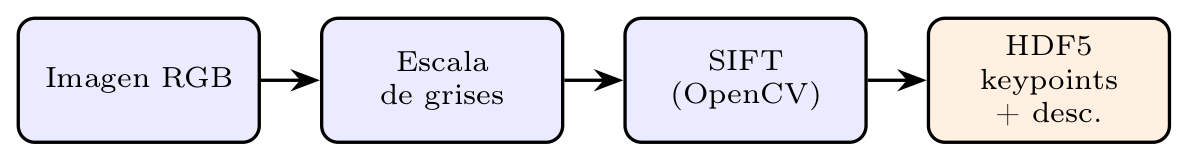
\includegraphics[width=0.72\textwidth]{16_diagramas_flujo/diagrama_sift.png}\\[0.6em]
  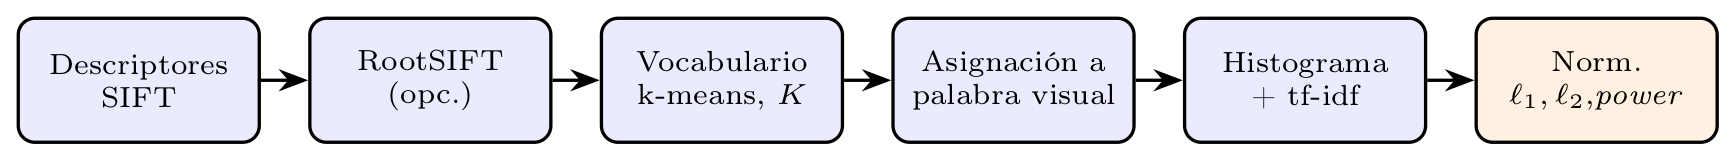
\includegraphics[width=0.9\textwidth]{16_diagramas_flujo/diagrama_bovw.png}\\[0.6em]
  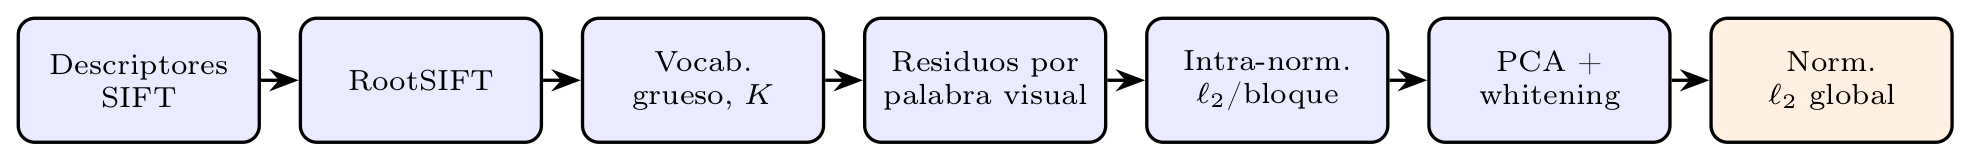
\includegraphics[width=0.9\textwidth]{16_diagramas_flujo/diagrama_vlad.png}
  \ideaclave{A partir de los mismos descriptores SIFT se construyen dos representaciones: BoVW (conteo) y VLAD (residuos).}
\end{frame}

% ============================================================================
\begin{frame}{Pipeline general (2/2): descriptores globales y ranking}
  \centering
  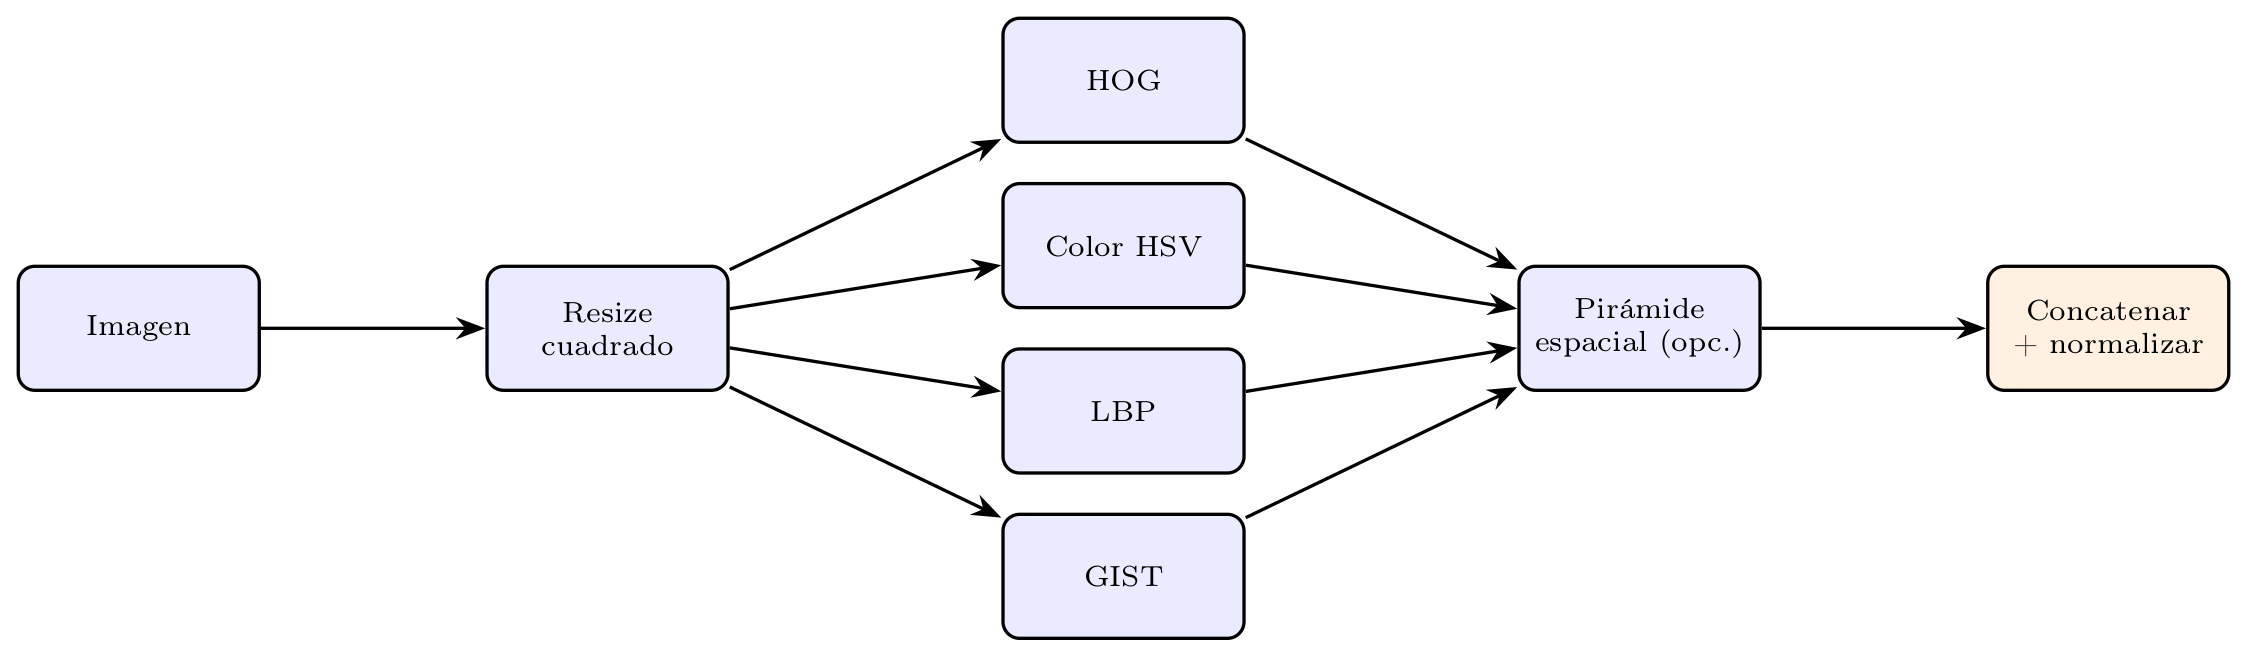
\includegraphics[width=0.85\textwidth]{16_diagramas_flujo/diagrama_descriptores_globales.png}\\[0.8em]
  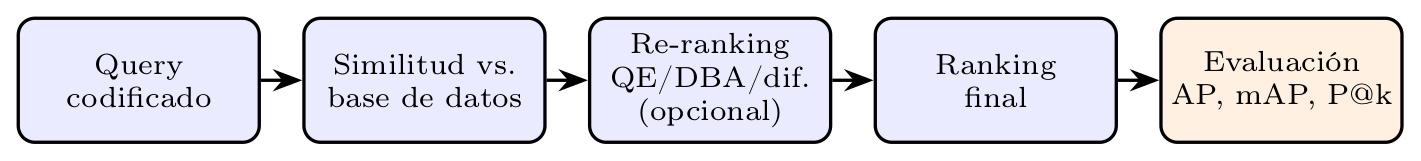
\includegraphics[width=0.72\textwidth]{16_diagramas_flujo/diagrama_retrieval.png}
  \ideaclave{Todos los m\'etodos terminan en un vector de longitud fija: eso permite comparar la consulta contra toda la base y producir un ranking.}
\end{frame}

% ============================================================================
\begin{frame}{SIFT y RootSIFT}
  \begin{columns}[T]
    \begin{column}{0.5\textwidth}
      \begin{itemize}
        \item SIFT detecta puntos estables en escala y orientaci\'on.
        \item Cada keypoint: vector de 128 valores.
        \item Descriptores guardados en HDF5 (no se recalculan).
        \item RootSIFT: normalizaci\'on $\ell_1$ + ra\'iz cuadrada.
      \end{itemize}
      \[
        x_{\text{root}} = \sqrt{\dfrac{x}{\lVert x \rVert_1}}
      \]
      \small
      \textbf{Por qu\'e SIFT:} robusto a escala, rotaci\'on y cambios moderados de iluminaci\'on.\\
      \textbf{Limitaci\'on:} detecta textura irrelevante (hojas, ramas).
    \end{column}
    \begin{column}{0.5\textwidth}
      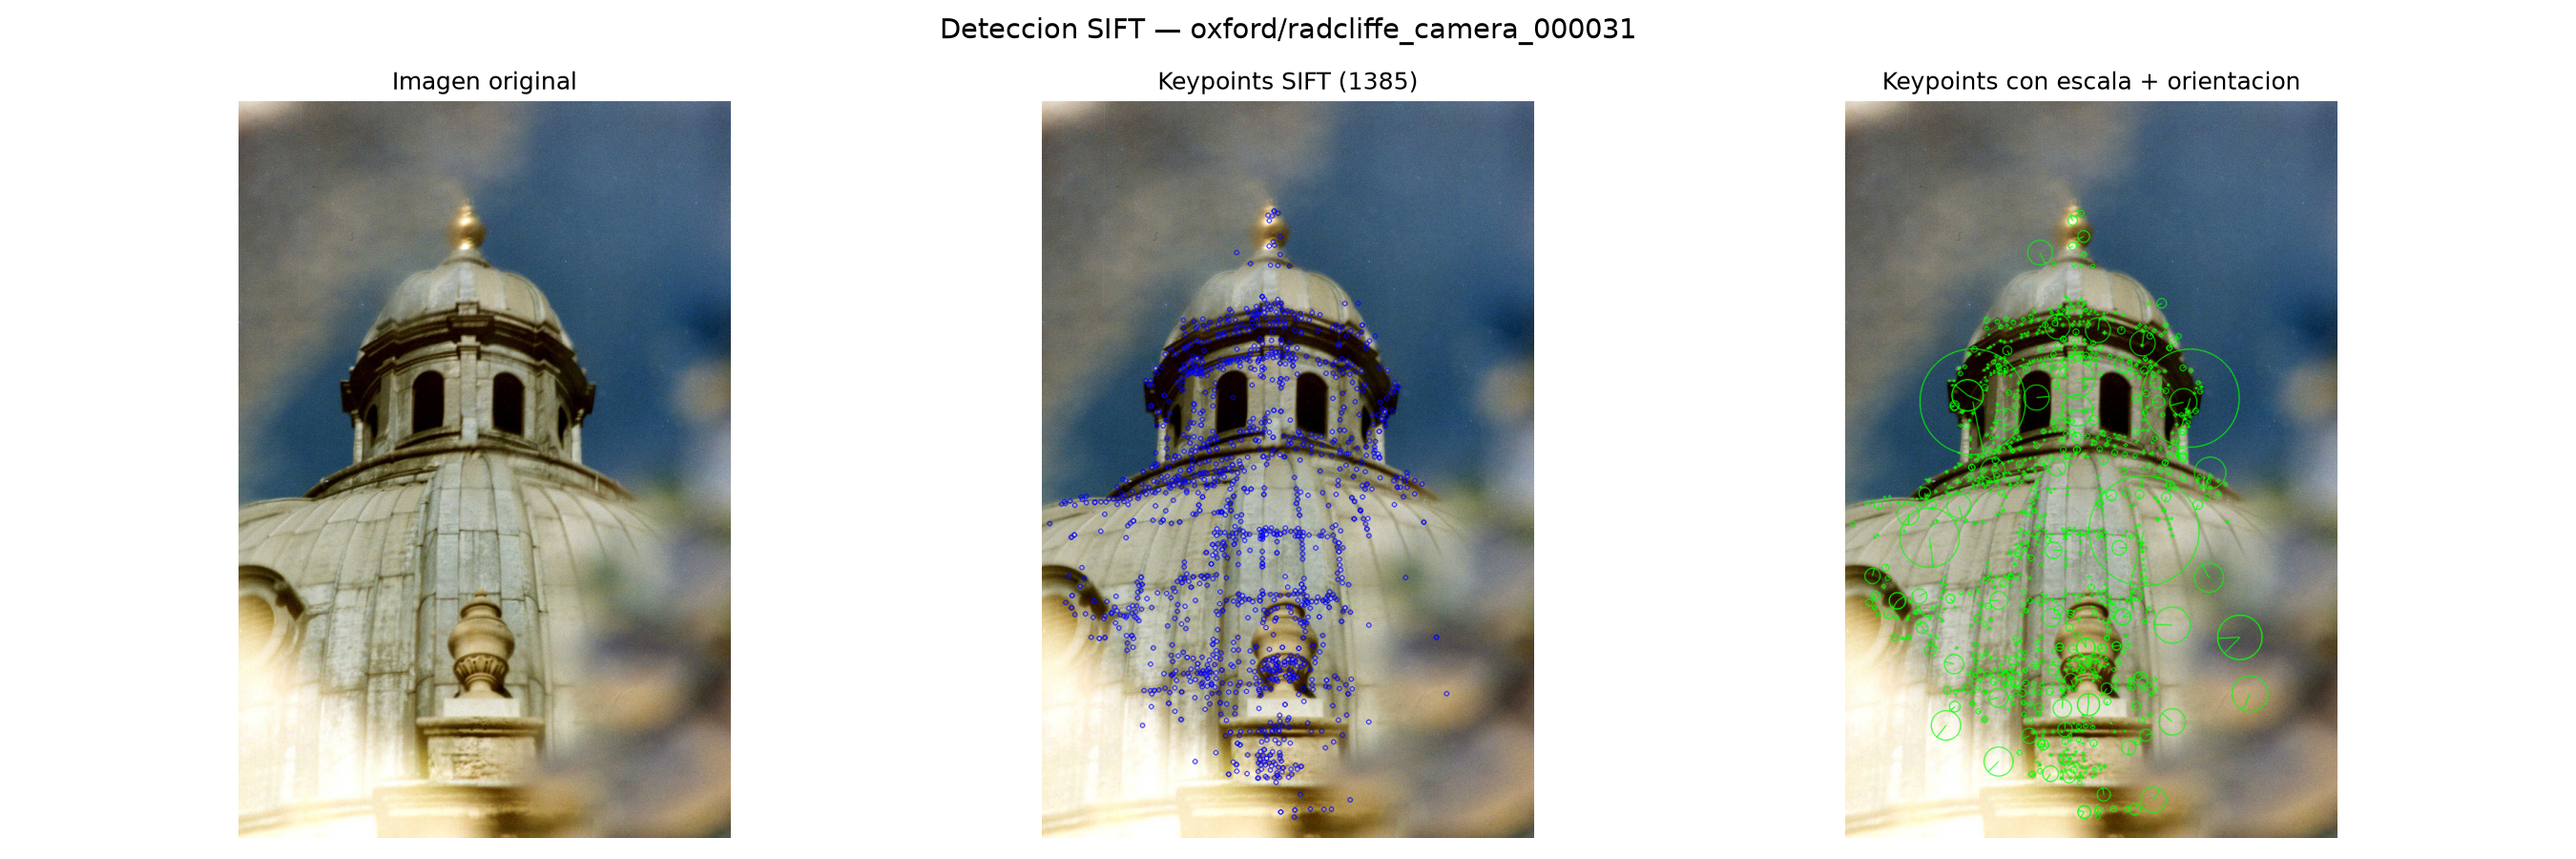
\includegraphics[width=\textwidth]{01_sift_keypoints/sift_pipeline_detalle.png}
    \end{column}
  \end{columns}
\end{frame}

% ============================================================================
\begin{frame}{BoVW y vocabulario visual}
  \begin{columns}[T]
    \begin{column}{0.52\textwidth}
      \begin{enumerate}
        \item Muestra de descriptores SIFT.
        \item K-means aprende $K$ palabras visuales.
        \item Cada descriptor $\rightarrow$ centroide m\'as cercano.
        \item Histograma de $K$ posiciones por imagen.
      \end{enumerate}
      \begin{center}
        \small descriptores SIFT $\rightarrow$ palabras visuales $\rightarrow [12, 4, 0, 31,\dots]$
      \end{center}
      \vspace{0.3em}
      \small\textbf{Config. recomendada:} $K{=}4096$, RootSIFT, TF-IDF, norm.\ $\ell_1$
    \end{column}
    \begin{column}{0.48\textwidth}
      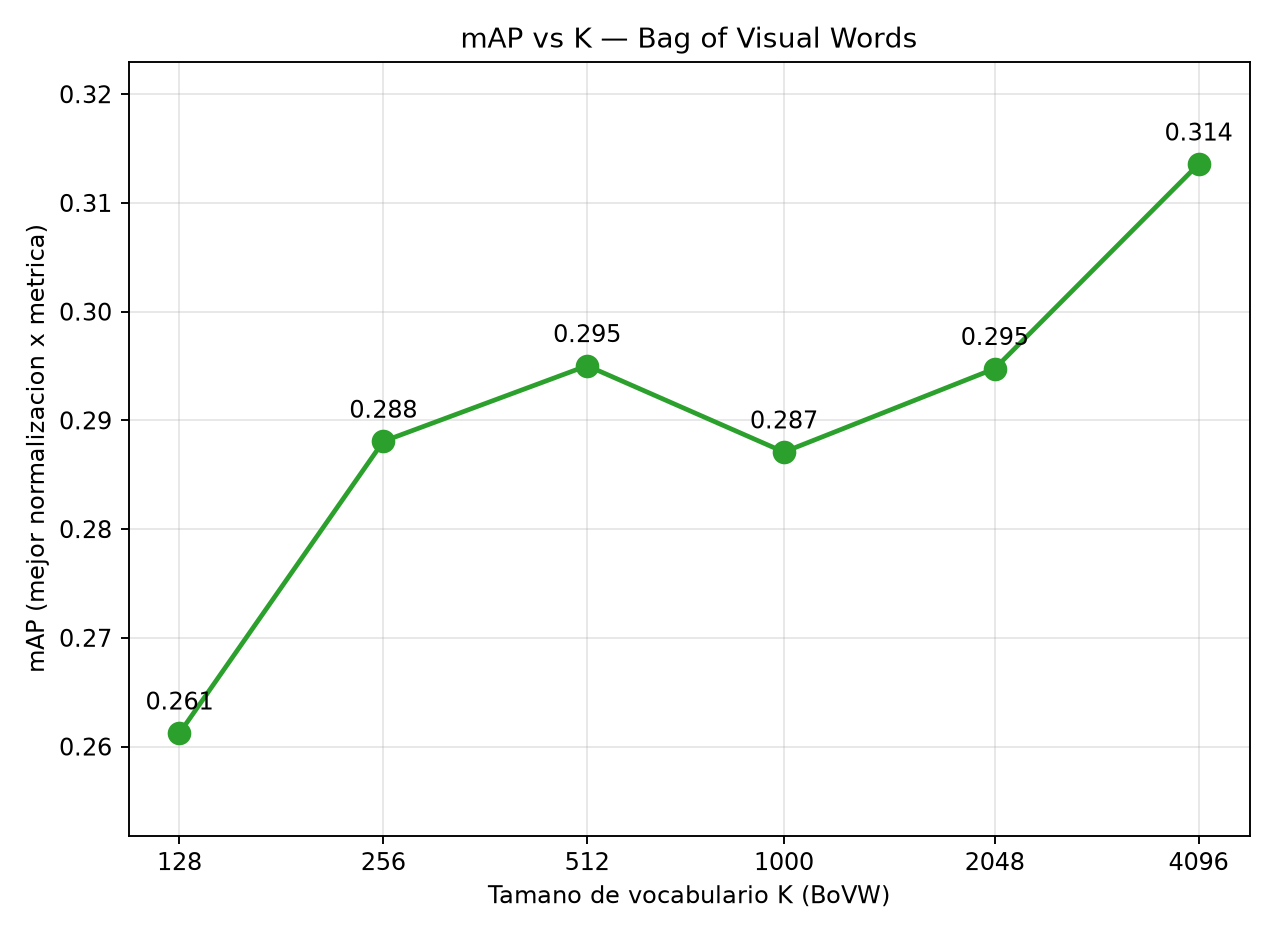
\includegraphics[width=\textwidth]{05_mAP_vs_K_bovw/mAP_vs_K_bovw.png}
    \end{column}
  \end{columns}
  \ideaclave{BoVW descarta la posici\'on espacial: dos edificios distintos pueden tener histogramas parecidos si comparten texturas.}
\end{frame}

% ============================================================================
\begin{frame}{Representaciones comparadas (mAP, Oxford)}
  \centering
  \begin{table}
    \scriptsize
    \begin{tabular}{lp{4.2cm}r}
      \toprule
      \textbf{Representaci\'on} & \textbf{Qu\'e conserva} & \textbf{mAP} \\
      \midrule
      Color (histograma HSV)                 & Distribuci\'on HSV                & 0.1049 \\
      LBP                                     & Textura                           & 0.1072 \\
      GIST                                    & Estructura global                 & 0.1427 \\
      HOG                                     & Bordes y forma                    & 0.1467 \\
      BoVW $K{=}4096$                         & Frecuencia de patrones locales     & 0.3136 \\
      VLAD $K{=}256$ + PCA                    & Residuos locales                  & 0.5282 \\
      \rowcolor{ProjLight}
      \textbf{VLAD + DBA + Difusi\'on}        & Residuos + re-ranking             & \textbf{0.7053} \\
      \bottomrule
    \end{tabular}
  \end{table}
  \ideaclave{Los descriptores globales son buenos baselines, pero el salto importante ocurre al modelar patrones locales: VLAD supera a BoVW porque conserva m\'as informaci\'on que un simple conteo.}
\end{frame}

% ============================================================================
\begin{frame}{VLAD y PCA whitening}
  \begin{columns}[T]
    \begin{column}{0.55\textwidth}
      VLAD acumula el residuo respecto al centroide asignado:
      \[
        v_k = \sum_{x \to c_k} (x - c_k)
      \]
      \begin{itemize}
        \item BoVW guarda \emph{cu\'antos} caen en cada centroide.
        \item VLAD guarda tambi\'en \emph{en qu\'e direcci\'on} se alejan.
      \end{itemize}
      \vspace{0.3em}
      \small
      \begin{tabular}{ll}
        $K$ & 256 \\
        RootSIFT & s\'i \\
        Intra-normalizaci\'on & s\'i \\
        PCA & 512 dim. \\
        whiten-power & 0.25 \\
      \end{tabular}
    \end{column}
    \begin{column}{0.45\textwidth}
      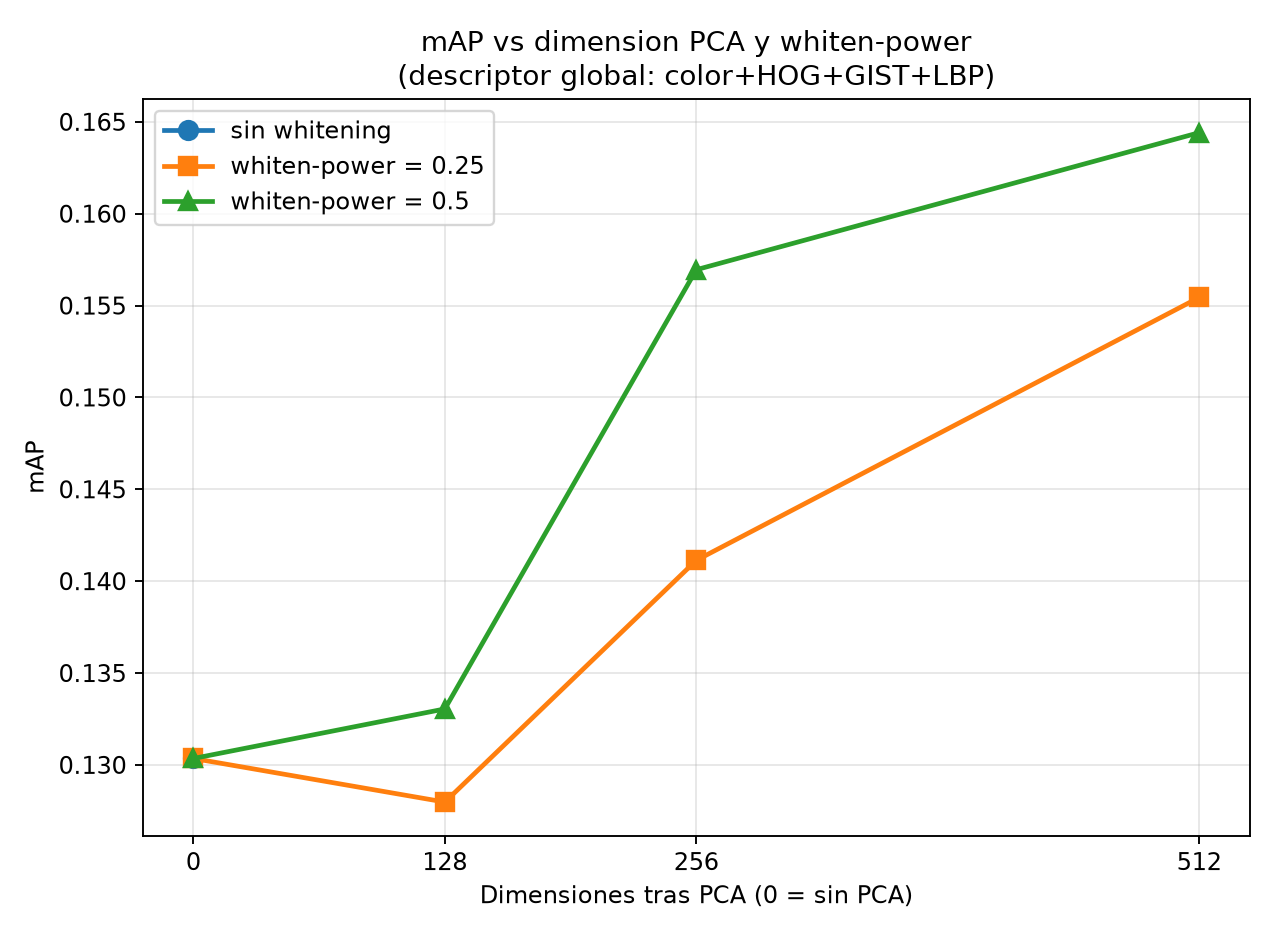
\includegraphics[width=\textwidth]{ppt_comparativas/pca_whitening_comparativa.png}
    \end{column}
  \end{columns}
  \ideaclave{PCA reduce dimensi\'on y correlaci\'on; la intra-normalizaci\'on evita que una textura repetitiva domine el vector.}
\end{frame}

% ============================================================================
\begin{frame}{Similitud y re-ranking}
  \textbf{Base:} similitud coseno entre vectores normalizados.
  \begin{columns}[T]
    \begin{column}{0.46\textwidth}
      \begin{itemize}
        \item \textbf{Query Expansion:} incorpora vecinos de la consulta.
        \item \textbf{DBA} ($n{=}5$): incorpora vecinos a cada vector de la base.
        \item \textbf{Difusi\'on} ($k{=}100$): propaga similitud por un grafo de vecinos.
      \end{itemize}
    \end{column}
    \begin{column}{0.54\textwidth}
      \scriptsize
      \begin{tabular}{lr}
        \toprule
        \textbf{Etapa} & \textbf{mAP} \\
        \midrule
        VLAD base                          & 0.5282 \\
        + Query Expansion                  & 0.5545 \\
        + DBA                              & 0.5817 \\
        + Difusi\'on                       & 0.6780 \\
        \rowcolor{ProjLight}
        \textbf{+ DBA(5) + Difusi\'on(100), seeds=5} & \textbf{0.7053} \\
        \bottomrule
      \end{tabular}
    \end{column}
  \end{columns}
  \ideaclave{La difusi\'on ayuda porque im\'agenes del mismo edificio forman una cadena de vistas parecidas, aunque dos de ellas no se parezcan directamente.}
\end{frame}

% ============================================================================
\begin{frame}[fragile]{Evaluaci\'on}
  \begin{columns}[T]
    \begin{column}{0.55\textwidth}
      \small
      \begin{block}{Precision@k}
        Fracci\'on de relevantes en los primeros $k$: \\
        $\text{Precision@k} = \dfrac{\text{relevantes en top-}k}{k}$
      \end{block}
      \begin{block}{AP y mAP}
        AP: calidad del ranking de una query.\\
        mAP: promedio del AP sobre todas las queries.
      \end{block}
    \end{column}
    \begin{column}{0.45\textwidth}
      \small
      \textbf{Protocolo:}
      \begin{itemize}
        \item Se eliminan las im\'agenes \texttt{junk}.
        \item Cada query se eval\'ua contra su propio dataset.
        \item Se usa la base completa (no solo top-5) para AP.
      \end{itemize}
    \end{column}
  \end{columns}
  \vspace{0.4em}
  {\tiny\ttfamily
  python 4\_evaluate\_retrieval.py --embeddings vlad\_k256\_pca512.npz \textbackslash\\
  \hspace*{2em}--name vlad\_best --metric cosine --datasets oxford \textbackslash\\
  \hspace*{2em}--dba 5 --diffusion 100 --diffusion-seeds 5
  }
\end{frame}

% ============================================================================
\begin{frame}{An\'alisis Oxford vs.\ Paris}
  \begin{columns}[T]
    \begin{column}{0.45\textwidth}
      \small
      \begin{tabular}{lrr}
        \toprule
        \textbf{Dataset} & \textbf{VLAD base} & \textbf{+DBA+dif.} \\
        \midrule
        Oxford & 0.5282 & 0.7053 \\
        Paris  & 0.5514 & \textbf{0.8119} \\
        \rowcolor{ProjLight}
        Oxford+Paris & -- & 0.7586 \\
        \bottomrule
      \end{tabular}
    \end{column}
    \begin{column}{0.55\textwidth}
      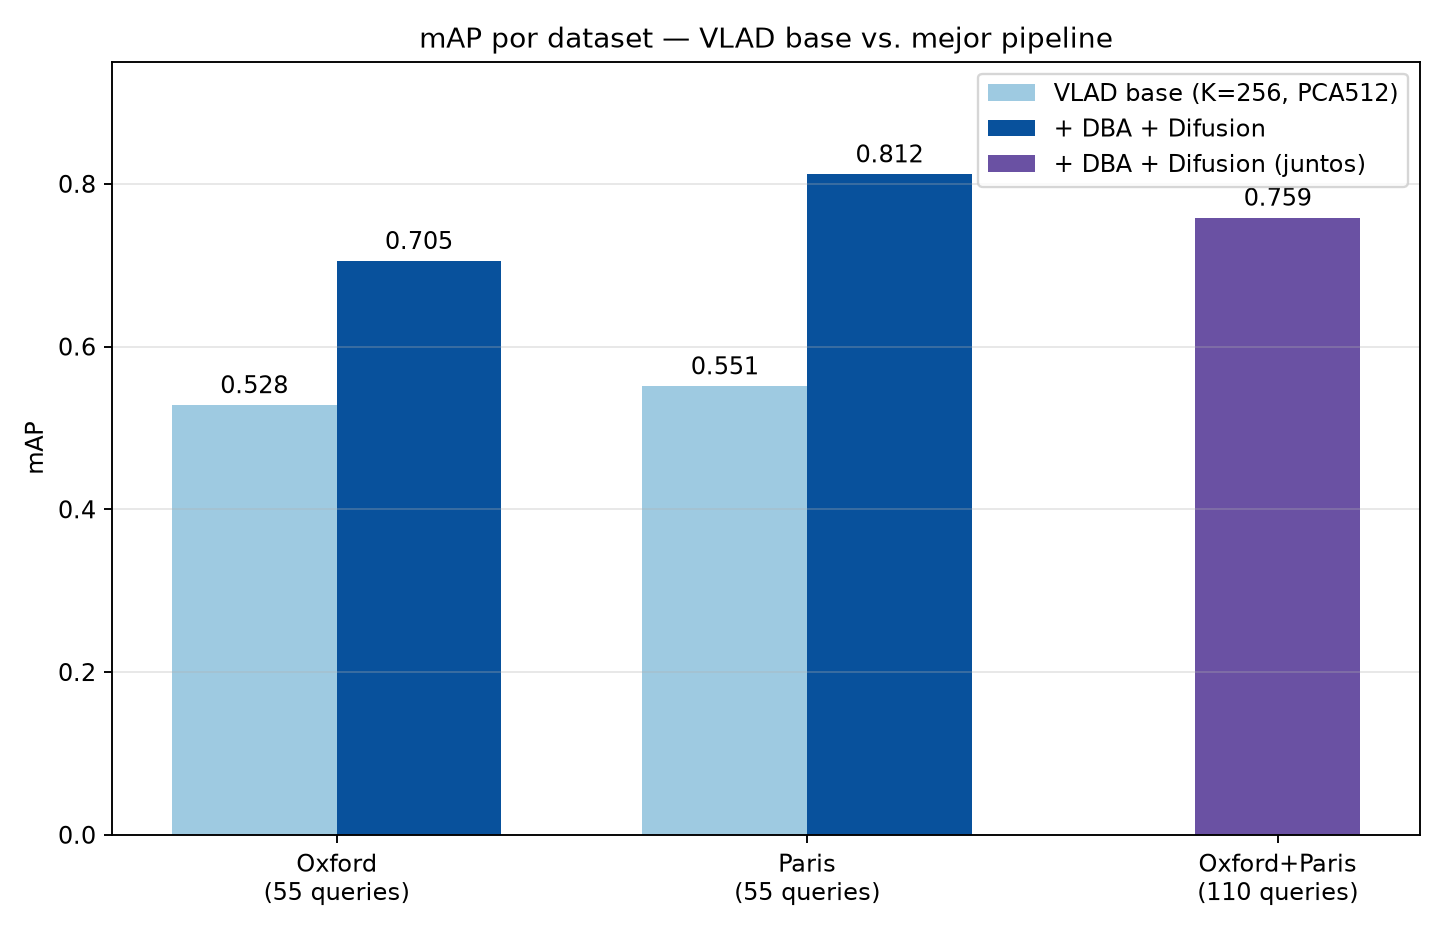
\includegraphics[width=\textwidth]{12_oxford_vs_paris/mAP_oxford_vs_paris.png}
    \end{column}
  \end{columns}
  \ideaclave{La mejora no es exclusiva de Oxford: tambi\'en se observa en Paris, lo que indica que el re-ranking generaliza dentro de este protocolo.}
\end{frame}

% ============================================================================
\begin{frame}{Caso exitoso}
  \centering
  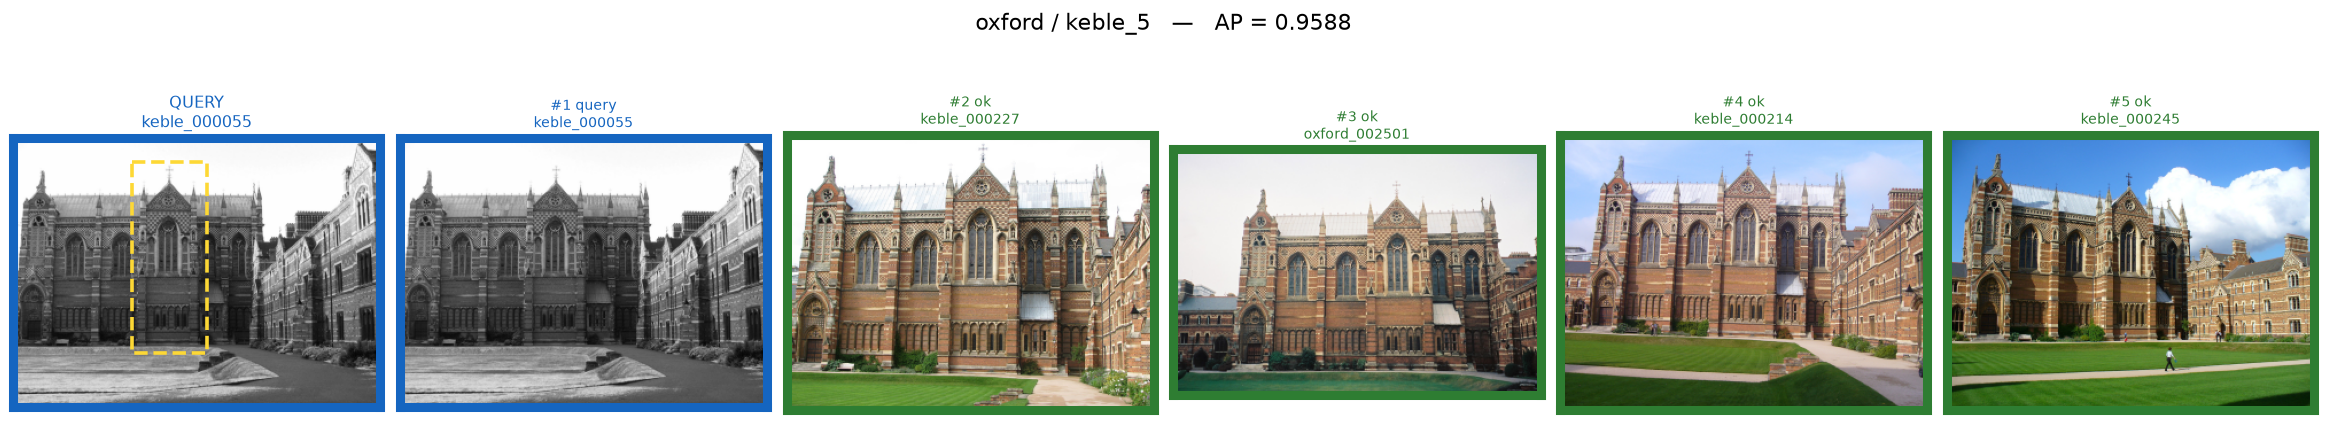
\includegraphics[width=\textwidth]{ppt_comparativas/vlad_best_case_2_keble_AP0.959.png}
  \vspace{0.5em}
  \small Vistas que comparten estructura de fachada: los patrones locales se mantienen pese al cambio de captura.
\end{frame}

\begin{frame}{Caso de fallo}
  \centering
  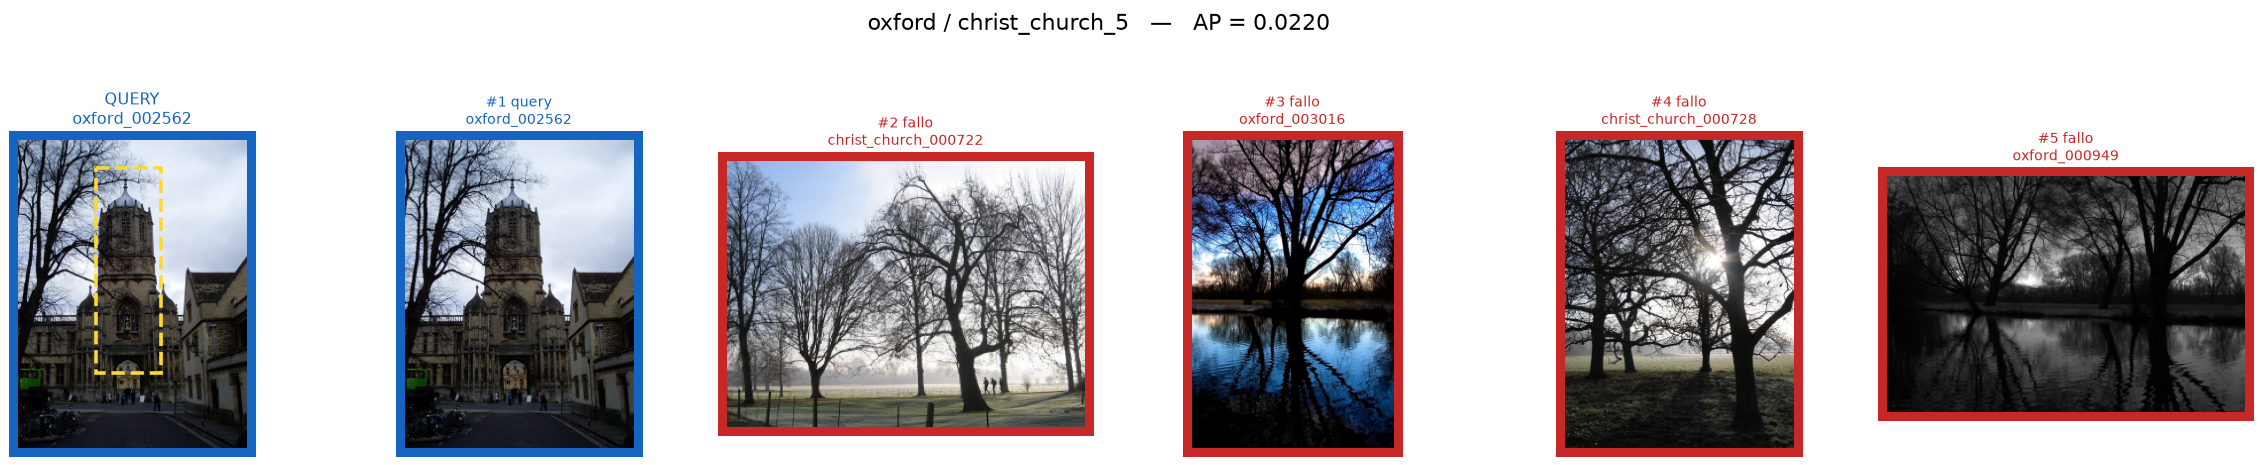
\includegraphics[width=\textwidth]{ppt_comparativas/vlad_failure_case_1_christchurch_AP0.022.png}
  \vspace{0.5em}
  \small Vegetaci\'on y fondos con textura producen descriptores parecidos a los de otros landmarks.
  \ideaclave{Magdalen es dif\'icil en casi todas las representaciones. El bbox puede ayudar cuando el edificio ocupa poca \'area, pero no siempre: eliminar demasiado contexto tambi\'en perjudica.}
\end{frame}

% ============================================================================
\begin{frame}{Conclusiones}
  \begin{enumerate}
    \item SIFT es una buena base para edificios: representa patrones locales.
    \item BoVW es eficiente, pero pierde informaci\'on espacial y de residuos.
    \item VLAD mejora claramente a BoVW.
    \item DBA y difusi\'on mejoran el ranking sin aprendizaje profundo.
    \item La evaluaci\'on combina mAP, Precision@k y ejemplos visuales.
  \end{enumerate}
  \vspace{0.5em}
  \textbf{Trabajo futuro:} verificaci\'on geom\'etrica (Lowe + RANSAC), uso sistem\'atico del bbox, ASMK/Fisher Vectors, indexaci\'on invertida.
  \ideaclave{Lo importante no es solo que VLAD tenga mayor mAP, sino entender por qu\'e: conserva informaci\'on que BoVW descarta, y el re-ranking explota la estructura de vecinos del conjunto.}
\end{frame}

% ============================================================================
\begin{frame}[plain]
  \begin{center}
    \Huge \textcolor{ProjBlue}{\textbf{Gracias}}\\[0.5em]
    \Large \textcolor{ProjBlue}{\textbf{Preguntas}}
  \end{center}
\end{frame}

% ============================================================================
% BACKUP
% ============================================================================
{
\setbeamercolor{background canvas}{bg=ProjLight}
\begin{frame}[plain]
  \begin{center}
    \Large\textbf{Backup: preguntas frecuentes}
  \end{center}
\end{frame}
}

\begin{frame}{Preguntas frecuentes (1/2)}
  \small
  \textbf{Por qu\'e BoVW no es suficiente?}\\
  Representa la imagen como histograma de frecuencias y pierde \emph{d\'onde} aparecen los patrones; VLAD conserva el residuo respecto al centroide.
  \vspace{0.4em}

  \textbf{Qu\'e significa $K$ en BoVW/VLAD?}\\
  N\'umero de centroides del vocabulario: bins del histograma (BoVW) o bloques de residuos (VLAD).
  \vspace{0.4em}

  \textbf{Por qu\'e un $K$ mayor no siempre es mejor?}\\
  Es m\'as discriminativo, pero necesita m\'as memoria y datos por cl\'uster; con pocos descriptores por cl\'uster el vocabulario se vuelve inestable.
\end{frame}

\begin{frame}{Preguntas frecuentes (2/2)}
  \small
  \textbf{Diferencia entre AP y mAP?}\\
  AP mide una query; mAP promedia el AP sobre todas las queries.
  \vspace{0.4em}

  \textbf{El resultado puede diferir de otra implementaci\'on?}\\
  S\'i: cambiar las queries, el uso del bbox, el tratamiento de \texttt{junk} o la f\'ormula de AP altera el mAP. Todos los modelos deben evaluarse con el mismo protocolo.
  \vspace{0.4em}

  \textbf{El re-ranking usa deep learning?}\\
  No. DBA y difusi\'on operan sobre vectores y grafos de similitud: son m\'etodos cl\'asicos y \emph{training-free}.
\end{frame}

\end{document}
